% !TEX root = main.tex

\section{简介}
自然语言处理(natrual language processing, NLP)又叫计算语言学,是研究如何利用计算机技术对语言文本(句子、篇章、话语等)进行加工处理的一门学科,包括对词法、句法、语义、语用等信息的识别、分类、提取转换和生成等各种处理方法和实现技术。
主要内容包括:机器翻译、信息检索、自动文摘、观点挖掘、问答系统、信息抽取、文档分类、文字编辑和自动校对、语音识别、文语转换、语音合成、说话人识别/认同/验证。

\subsection{基本问题与主要困难}
\subsubsection{基本问题}
\begin{itemize}
\item 形态学(morphology):词由有意义的基本单位---\textbf{词素}(词根、前缀、后缀、词尾)的构成问题、单词识别/汉语分词问题
\item 句法(syntax)问题:研究句子结构成分之间的相互关系和组成句子序列的规则(\textbf{主谓宾})
\item 语义(semantics)问题:研究如何从一个语句中推导出词的意义,以及这些词在语句句法结构中的作用来推导出该语句的意义(同一个词在不同语境下会有\textbf{不同意思})
\item 语用学(pragmatics):研究在不同上下文语句的应用,以及上下文对语句理解产生的影响
\end{itemize}

\subsubsection{主要困难}
\begin{itemize}
	\item 大量\textbf{歧义}:
	\begin{itemize}
		\item 词法歧义
		\begin{displayquote}
		研究所/取得\\
		研究/所取得
		\end{displayquote}
		\item 词性歧义
		\begin{displayquote}
		动物保护警察\\
		Time flies like an arrow.
		\end{displayquote}
		\item 结构歧义
		\begin{displayquote}
		今天中午吃\underline{馒头}\\
		今天中午吃\underline{食堂}\\
		I saw [a man with a telescope].\\
		I [saw a man] with a telescope.
		\end{displayquote}
		\item 语义歧义(缩略语、隐喻)
		\begin{displayquote}
		意思意思是几个意思?
		\end{displayquote}
		\item 语音歧义
	\end{itemize}
	\item 大量\textbf{未知语言现象}:新词、人名、地名、术语、新含义、新句法、新句型
\end{itemize}

\subsection{信息论基础}
\begin{figure}[H]
\centering
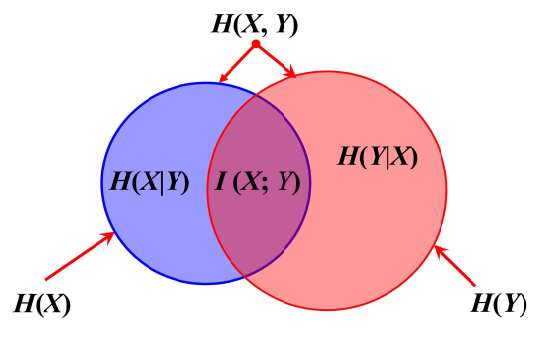
\includegraphics[width=0.4\linewidth]{fig/entropy.png}
\end{figure}
\begin{definition}[熵/自信息]
概率分布为$p(x)=P(X=x)$,则熵$H(X)$为
\[H(X)=-\sum_{x\in X}p(x)\log_2p(x)\]
并约定$0\log 0=0$,单位为二进制位比特(bit)
\end{definition}
\begin{definition}[联合熵]
$X,Y$为离散型随机变量$X,Y\thicksim p(x,y)$,联合熵定义为
\[H(X,Y)=-\sum_{x\in X}\sum_{y\in Y}p(x,y)\log_2 p(x,y)\]
是描述一对随机变量平均所需的信息量
\end{definition}
\begin{definition}[条件熵]
\[H(Y\mid X)=-\sum_{x\in X}\sum_{y\in Y}p(x,y)\log_2 p(y\mid x)\]
\end{definition}
\begin{definition}[相对熵(KL距离)]
两个概率分布$p(x)$和$q(x)$的相对熵定义为
\[D(p||q)=\sum_{x\in X}p(x)\log_2\frac{p(x)}{q(x)}\]
注意\textbf{相对熵没有负号}!
\end{definition}
\begin{definition}[交叉熵]
若随机变量$X\thicksim p(x)$,$q(x)$用于近似$p(x)$的概率分布,则$X$与模型$q$的交叉熵定义为
\[H(X,q)=H(X)+D(p||q)=-\sum_x p(x)\log_2 q(x)\]
其常用来衡量估计模型与真实概率分布之间的差异
\end{definition}
\begin{definition}[互信息]
如果$(X,Y)\thicksim p(x,y)$,则$X,Y$之间的互信息$I(X;Y)$定义为
\[I(X;Y)=H(X)-H(X\mid Y)=\sum_{x\in X}\sum_{y\in Y}p(x,y)\log_2\frac{p(x,y)}{p(x)p(y)}\]
互信息值越大,表示两个汉字之间的\textbf{结合越紧密},越有可能成词。
\end{definition}

\begin{example}[基于上下文分类的消歧方法]
基于贝叶斯分类器,假设某个多义词$w$所处上下文语境为$C$,其多个语义为$s_i$,则可以通过计算
\[\argmax_{s_i} p(s_i\mid C)=\argmax_{s_i}\lrs{\log p(s_i)+\sum_{v_k\in C}\log p(v_k\mid s_i)}\]
确定词义。
由统计数据可得
\[\begin{aligned}
p(v_k\mid s_i)&=\frac{N(v_k,s_i)}{N(s_i)}\\
p(s_i)&=\frac{N(s_i)}{N(w)}
\end{aligned}\]
其中$N(s_i)$为训练数据中词$w$用于语义$s_i$时的次数,而$N(v_k,s_i)$为$w$用于语义$s_i$时词$v_k$出现在$w$的上下文中的次数,$N(w)$为$w$在训练数据中出现的总次数。
\end{example}

\subsection{语言学基础}
\begin{definition}[词性(parts of speech, POS)/句法类/语法类]
相似的语法结构行为和典型的语义类型聚成不同的类,称为词性。
\end{definition}
\begin{definition}[词法]
词法则是构词过程,包括\textbf{变形}(修改时态、数目等)、\textbf{派生}、\textbf{复合}。
\end{definition}

短语结构可通过树来表达
\begin{center}
[S[NP[AT The][NNS children]][VP[VBD ate][NP[AT the][NN cake]]]]
\end{center}

主要汉字编码标准:ASCII(英文)、GB2312(中文)、BIG5(繁体)、Unicode(统一编码)。

UTF(Unicode Transformation Format)是Unicode的实现方式,从Unicode码点到唯一字节序列的映射算法,一一映射,保证无损转换。